\documentclass[12pt]{article}
\usepackage{fullpage}
\usepackage{times}
\usepackage{cite}
\usepackage{hyperref}
\usepackage{algorithmic}
\usepackage[top=2.4cm, bottom=2.4cm, left=2.4cm, right=2.4cm]{geometry}
\usepackage[center]{figbib}

\usepackage{amssymb}
\usepackage{algorithm}
\usepackage{adjustbox}
\usepackage{graphicx}
\usepackage{pdfpages}





\linespread{1.25}

\newcommand{\code}[1]{\texttt{#1}}
\begin{document}

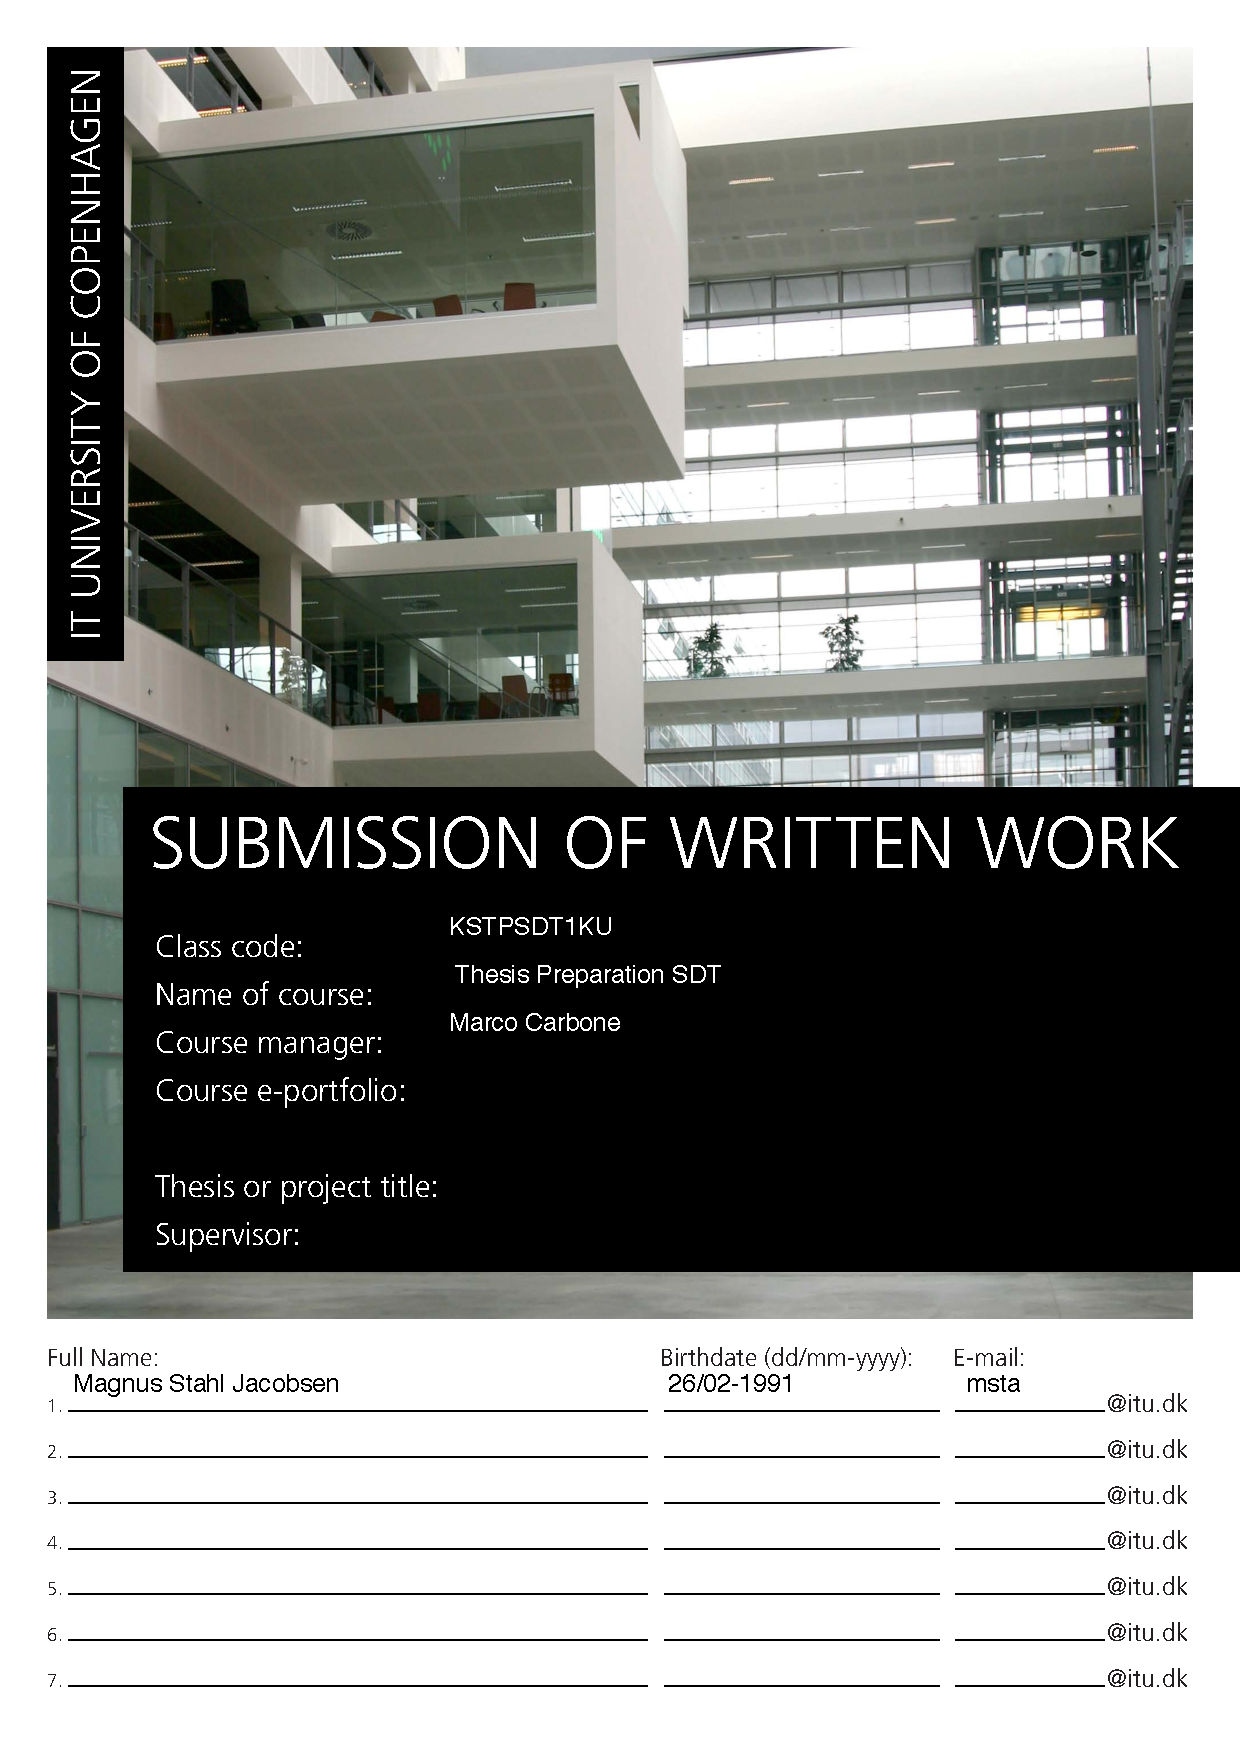
\includepdf[pages={1}]{front.pdf}



\begin{center}
    \vspace{2cm}
    \huge { Thesis Preparation Report \\ }
    \vspace{2cm}
    \large {Magnus Stahl (msta@itu.dk)\\
    IT-University of Copenhagen\\
    Fall 2016\\}
    \large {Supervisor: Natalie Schluter\\}
\end{center}


\tableofcontents

\newpage

    
\section{Introduction}
\label{intro}

This report details introductory thesis work as part of a spring 2017 thesis at the IT-University of Copenhagen. The report will describe the work undertaken so far, and a plan for how the thesis will be completed in the spring. \\

The thesis I will write is placed in the field of Natural Language Processing, and more specifically Natural Language Understanding. Natural Language Understanding is the subject of making computers understand human language, possibly on the same level as humans. The subject can be investigated in a strong or weak AI perspective. This either entails trying to create a general idea of intelligence (strong AI) or splitting the language understanding task into smaller subtasks which can then be solved. My thesis will be placed in the latter category. I will look only at sentence level language understanding. Understanding a sentence is a task also composed of many other subtasks, from spelling individual words and understanding the meaning, recognizing composite words, understanding how each word relate to the sentence and abstracting higher meanings from the sentence. I will look at the task of \emph{classifying} relations between entities (usually nouns) in a sentence. Classification of relations in sentences are important because relations are a central component in the higher meaning for a sentence. Classification in this context means mapping sentences and their entities to a category which explains the nature of the relationship between them. \\
Classification is most commonly solved with machine learning, which in this case entails looking at a set of sentences with known relations, and then extracting patterns automatically from these samples. 

The task of relation classification can be more formally defined as:
Given a sentence $S$ and two labeled entities textless e1\textgreater and \textless e2\textgreater, classify the relation between the entities and (optionally) the ordering of the relation. Here is an example:

\begin{center}

$S$: \emph{``The train rolled onto the platform with a peculiar choo choo.''} \\

\textless e1\textgreater: \emph{train} \\
\textless e2\textgreater: \emph{platform} \\

Relation: \emph{Entity-Destination(e1,e2)}

\end{center}

Many classes of algorithms exists for solving classification tasks, but in my thesis I will focus on neural networks.
Artificial Neural Networks (ANN) are a group of data structures and related algorithms that loosely models features of a biological brain. ANNs can be used for a wide variety of machine learning tasks such as text analysis, speech recognition and computer vision. The last 10 years have witnessed a great increase in the use of neural networks due to multiple factors such as increased computing power and parallel capabilities with mainstream GPU's. Another factor is the work of specific research groups on new neural network patterns such as Long-Short-Term-Memory or Convolutional Neural Networks by the IDSIA group \cite{idsa}.

In my thesis, I will investigate contemporary neural networks used for solving the relation classification task. I will try to recreate some of the results claimed by the creators of those networks by re-implementing the networks with modern deep learning frameworks. Then I will investigate the state-of-the-art approaches and experimentally find out if the same results may be achieved with a simpler network. I will try to investigate why certain approaches are suggested and try to separate parts of the network structure which is badly (or perhaps un-)motivated. I will use a common dataset (SemEval 2010, task 8) to document the results. And finally, if time allows it, I will perhaps look at relation classification in a domain-based space where the relations to be classified are very specific to the individual domain. 


\subsection{Research questions}

I have formulated the following tentative research questions:
\begin{itemize}
    \item What are the current state-of-the-art systems for relation classification 
    with neural networks?\\
    \item Is it possible to simplify structures in state-of-the-art systems while maintaining (or increasing) the F1 metric?
\end{itemize}


\begin{center}
\fbEpsfig{cnn_fig}{\textwidth}{htbp}
\end{center}


\subsection{Motivation}

This section motivates why the subject of the thesis is important.\\

Relation classification is a hard task for computers. Correctly classifiying entities in language requires understanding the context of the entities as well as an abstract understanding
of their relationship. Recent deep learning experiments have yielded excellent results compared to feature-based classifiers, which require feature engineering.  Neural networks are interesting in NLP because they allow features to be learned automatically from raw input data. This can lower the entry barrier for working with language systems as features usually require linguistic domain knowledge.  

Simplification of state-of-the-art systems, and especially neural networks, is interesting because the newest systems are often built on top of other state-of-the-art systems. These ``research iterations'' often
lead to including substructures from previous systems which might not be relevant in the newer system. Additionally, hyperparameters are not always decided by search but rather by sticking to values which were chosen in a previous system. Hyperparameters might incur unnessecary memory or performance costs. Finally, many paper suggest that simpler networks reduce overfitting and thus generalize better \cite{dropout}.



\section{Work so far}

This section details how I have been preparing for the thesis until January 2017.
I will begin by detailing the literature I have followed to learn more about the subject.

\subsection{Preparation}
I have before the start of the 2016 fall semester completed courses in mathematics (msc level), data mining and intelligent systems. I have written a bachelors thesis on the subject of classification and prediction.\\

In the thesis preparation course, I have learned more about deep learning and NLP. I have completed
a small deep learning course on Udacity\cite{udacity}.
To complement the general deep learning knowledge I have started to read an MIT newly released 
grad level book about deep learning\cite{dlbook}

To connect my knowledge about machine learning with natural language processing, I started with Yoav Goldberg's tutorial about Deep Learning in NLP (reference). I have followed a coursera course on Natural Language Processing from Columbia University which details the more traditional approaches to NLP tasks. I have attended a NLP workshop on structured prediction in Named Entity Recognition and Part-Of-Speech tagging. 

Finally I have researched the algorithms behind word embeddings which are a commonly used tool when transforming text input to real-valued vectors. The word embedding algorithms which I have investigated (and which are also used in the baseline) are the skip-gram and the word2vec model\cite{skipgram}.

\subsection{Work}
Now I will describe the work I have done on the first research question described in section \ref{intro}.

I have researched which research papers claims state-of-the-art performance on the relation classification task. Most papers use a convolutional structure as the base structure of the network. Several papers in the last two years have claimed a new F1 score record on the SemEval 2010 task 8 dataset. I have implemented a few of those\cite{att_cnn}\cite{re_cnn} and read others who have similar scores with slightly different approaches (other papers here). The papers might differ in their use of loss function, input representation, values of hyperparameters and training algorithms.

I have also read a paper detailing the use of LSTM structures as their base structure\cite{re_lstm}. Some papers differ slightly in their objective (another common objective is relation extraction, in which the entities are not known as part of the input).

I have implemented these novel networks in Keras, a deep learning framework which uses TensorFlow as backend\cite{keras}\cite{tensorflow}.  

\newpage

\section{Thesis plan}

This sections details my plan for the thesis. 
During the entire project I plan to have weekly meetings with my supervisor. Before starting the thesis, I will
also revise the project agreement so it encompasses the experiences I have gathered during the thesis preparation course. 

I will now briefly outline the overall plan and then go into details with each step.
Shown below is a Gantt chart which details the overall plan:

\begin{center}
\fbEpsfig{gantt}{\textwidth}{htbp}
\end{center}

As shown on the chart, I have divided my work in 7 parts, which will be done in four timespans.

\subsection{Initial research}
 The first few weeks of the project will be used on additional preliminary reading and finishing the investigation on current state-of-the-arts systems.
The conclusion of the investigation will be an outline of a system that will serve
as my baseline for future experimentation and simplification. 

\subsection{Baseline implementation and method}
The next part of the project is designated to be roughly one month in length. The primary goal is to write the part of the report that details the related works (which I know about from the baseline investigation) and implement the baseline implementation. The end product (except from the report) of this part is a working baseline that is on-par with the current state-of-the-art systems. In this part I will also work on a method for simplifying the existing implementations. 

\subsection{Experimentation}
The third timespan of the project will be spent on simplifying current state-of-the-art systems. I will investigate different substructures of the proposed networks in terms of their motivation and impact on the result. For the experimentation I will use a server which is provided by the NLP group at ITU. The server provides the necessary GPU to efficiently parallelize neural network computations.  

\subsection{Write up, report}
The final part of the project will be focused on writing a good report. While I will write the report during the rest of the project as well, a final month of focusing on detailing everything correctly seems necessary. In this period I will also have time to properly document and illustrate the (potentially) new structure I have created. 
Finally, I am reserving the last week of the project for proof-reads.


\section{Conclusion}
This section concludes my report. I have detailed the objective of the thesis and motivated why it is important. I have placed the subject of the thesis in the area of science where it belongs. I have formulated tentative research questions and defined the task which I'm trying to solve formally. I have detailed the prepatory work I have done as part of the course, and finally I have detailed the plan of the full thesis project.


\bibliographystyle{apalike}
\bibliography{Bibliography}

\fbList{figures.bib}
    
\end{document}

    